\chapter{Usage of the Hybrid Fortran Framework} \label{cha:usage}

This chapter is intended to give the informations necessary for installing and using the \textbf{Hybrid Fortran} framework.

\section{Framework Dependencies} \label{sec:dependencies}

\textbf{Hybrid Fortran} requires the following software components:

\begin{enumerate}
 \item A compiler for either OpenACC Fortran or CUDA Fortran (PGI Accelerator v16.5 recommended).
 \item An x86 Fortran compiler.
 \item Python v2.6.x, Python v2.7.x or compatible.
 \item GNU Make 3.81.
 \item GNU gcc or clang (aliased to gcc).
 \item A POSIX compatible operating system.
 \item (optional) \verb|valgrind| is recommended if you would like to use the test system shipped with this framework (accessible through \verb|make tests|).
 \item (optional) Allinea DDT if you need parallel debugging on the device.
 \item (optional) For the graphical callgraph representation using \verb|make graphs|: ``pydot'' python library\footnote{http://code.google.com/p/pydot/} as well as the ``Graphviz'' program package\footnote{http://www.graphviz.org/Download..php}.
 \item (optional) \verb|NetCDF4-Python| and \verb|numpy| in case you'd like to use Hybrid Fortran's automated testing together with NetCDF Output.
\end{enumerate}

\section{User Defined Components} \label{sub:userDefined}

The following files displayed in figure \ref{figure:hybridCUDAComponentsAndInfoFlow} are defined by the user:

\begin{description}
 \item[h90(H90) Fortran sources] A source directory that contains Hybrid Fortran files (h90/H90 extension). It may also contain files with f90 or F90 extensions. The source directory is by default located at \verb|path-to-project/source/*| (this can be changed in the \verb|path-to-project/config/MakesettingsGeneral| file).
 \item[Makefile] Used to define module dependencies. The Makefile is by default located at \verb|path-to-project/buildtools/Makefile|. Note: All source files are being copied into flat source folders before being compiled - the build system is therefore source directory structure agnostic, i.e. files can be placed into arbitrary subdirectores below the source directory.
  \item[MakesettingsCPU] CPU compiler settings are specified in \verb|MakesettingsCPU|, located at \verb|path-to-project/buildtools/|.
  \item[MakesettingsGPU] GPU compiler settings are specified in \verb|MakesettingsGPU|, located at \verb|path-to-project/buildtools/|.
  \item[MakesettingsGeneral] Common settings, such as executable file names, the choice Hybrid Fortran preprocessor implementation class, or files and folders being excluded from compilation. With the helper comments these settings should be self explanatory.
 \item[storage\_order.F90] This fortran file contains fortran preprocessor statements in order to define the storage order for both CPU and GPU implementation. It can be placed anywhere in the source directory or its subdirectories (see above).
\end{description}

\section{Build Interface} \label{sub:buildInterface}

\begin{description}
 \item[make] builds both cpu and gpu versions of the codebase situated in \linebreak\verb|path-to-project/source/*|.
 \item[make build\_cpu] builds the cpu version of the codebase situated in \verb|path-to-project/source/*|.
 \item[make build\_gpu] builds the gpu version of the codebase situated in \verb|path-to-project/source/*|.
 \item[make install] builds both cpu and gpu versions of the codebase situated in \verb|path-to-project/source/*| and installs the executables into the test folder defined in \verb|path-to-project/buildtools/MakesettingsGeneral|.
 \item[make install\_cpu] Like \verb|make install|, but only for the cpu version.
 \item[make install\_gpu] Like \verb|make install|, but only for the gpu version.
 \item[make clean] Removes the build directories as well as cpu executables from the test folders.
 \item[make clean\_cpu] Like \verb|make clean|, but only for the cpu version.
 \item[make clean\_gpu] Like \verb|make clean|, but only for the gpu version.
 \item[make tests] Executes \verb|make install| and runs the automatic tests (see sec. ~\ref{sec:testSystem}) for all executables.
 \item[make tests\_cpu] Like \verb|make tests|, but only for the cpu version.
 \item[make tests\_gpu] Like \verb|make tests|, but only for the gpu version.
 \item[make TARGETS DEBUG=1] builds TARGETS in debug mode (use any of the targets defined above). Uses the \verb|DebugCUDAFortranImplementation| in case of GPU compilation (by default), which prints predefined data points for every kernel parameter after every kernel execution. See also the flag \verb|DEBUG_MODE| in \verb|MakesettingsGeneral| which allows to use the debug mode by default.
 \item[make TARGETS VERBOSE=1] builds TARGETS with more detailed output.
 \item[make graphs] creates the graphical callgraph representations in the \linebreak\verb|path-to-project/build/callgraphs/| directory.
\end{description}

\section{Test Interface} \label{sec:testSystem}
\textbf{Hybrid Fortran} comes with an automated test system that - once set up - is intended to find all errors in your code, each time a build completes. This includes
\begin{itemize}
 \item Program errors - e.g. use \verb|stop 2| in your code in order to signal Hybrid Fortran that your program has reached a failure condition. This will lead \verb|make tests| to fail.
 \item Initialization errors (symbols / arrays being read without initializing them first), using \verb|valgrind|.
 \item Memory handling errors (in case you forget to deallocate arrays), using \verb|valgrind|.
 \item Computational errors, using reference data. Currently supported for this validation is output in \verb|NetCDF| format as well as standard Fortran \verb|.DAT| files. For NetCDF, up to five data dimensions per variable are supported, for .DAT files it is up to three dimensions.
\end{itemize}

\subsection{Remote Execution}
It is possible to run your tests remotely by putting the hostname or IP address into the environment variable \verb|HF_RUN_OVER_SSH|. This will run executables with the command \verb|ssh ${HF_RUN_OVER_SSH} [command]| instead of directly.

\subsection{Output Validation} \label{sub:testIntegration}
If you would like to integrate the provided output validation system, please do the following:
\begin{enumerate}
  \item \label{enum:writeProc} Choose between the following options for your output.
    \begin{enumerate}
      \item Have your program output in NetCDF format. In that case you will need \verb|numpy| as well as \verb|NetCDF-Python| installed as additional dependencies. It is recommended to install these dependencies into a \verb|virtualenv| such that you can use a different compilers for the post processing as for the program itself (you will need NetCDF compiled in both versions). Compiling the entire post processing stack with PGI compilers (all of python, numpy) is not recommended. You can then use the \verb|SOURCE_THIS_BEFORE_TESTING| and \verb|SOURCE_THIS_AFTER_TESTING| options in \verb|MakesettingsGeneral| to specify the activate and deactivate scripts for your virtualenv. In case of NetCDF, the Hybrid Fortran test system will automatically pick up any variable in your output and test it against the reference.
      \item Add calls to the \verb|helper_functions| module procedures \verb|write1DToFile|, \verb|write2DToFile| and \verb|write3DToFile| to your program to be tested in order to write your data to the \verb|.dat| files in the \verb|test\your-executable\out| folder. The \verb|helper_functions| module is part of the Hybrid Fortran libraries and it is always included in Hybrid Fortran builds - in fact it gets copied into your build directories for consistancy reasons. You may choose any filename for the \verb|.dat| files, the \verb|allAccuracy.py| script will find them automatically in the \verb|test\your-executable\out| folder.
    \end{enumerate}
  \item \label{enum:testCompile1} Compile (\verb|make; make install| in project directory) and run your program to make sure the files are being created. Make sure that they actually contain data, for example by checking the file size.
  \item Repeat steps \ref{enum:writeProc}, \ref{enum:testCompile1} in your reference source code in case you go for the .DAT-files option.
  \item Compress the reference data created by your reference program into \linebreak\verb|./test/your-executable/ref.tar.gz|. See also the description of \verb|runTest.sh| in conjunction with the \verb|validation| command below to understand the correct format.
  \item During development of your hybrid codebase, set the flags \verb|TEST_WITH_EVERY_BUILD| and \verb|DEBUG_MODE| to \verb|true| in the file \verb|MakesettingsGeneral|. This ensures that your tests will run with every build of Hybrid Fortran.
\end{enumerate}

\subsection{Interface} \label{sub:testInterface}
The following files are part of the sample test interface provided with \textbf{Hybrid Fortran}. They are located in the framework's binary directory. In order to set up the test system correctly, what's relevant for you is the information provided for the files \verb|runTest.sh| and \verb|runTests.sh|. The other files are described here for completeness and in case you'd like to adapt the system for different use cases.

\begin{description}
 \item [accuracy.py] Compares one NetCDF - or Fortran 90 \verb|.dat| file with a reference file. Endianness, number of bytes per floating point value can be specified for the \verb|.dat| case using command line parameters. See \verb|--help| for usage.
 \item [allAccuracy.sh] Compares all Fortran 90 \verb|.dat| files or NetCDF files according that match a filename pattern. By default, the pattern \verb|./out/*.dat| is used - you can override this by defining \verb|TEST_OUTPUT_FILE_PATTERN| in MakesettingsGeneral.
 \item [runTest.sh] Executes a series of tests for one executable. In order to use this, please \verb|cd| into the executable's test directory first. This script takes three mandatory and three optional command line arguments :
  \begin{enumerate}
   \item The path to the executable as seen from its working directory.
   \item The architecture name for which the tests should be performed (currently either \verb|cpu| or \verb|gpu|).
   \item The postfix of the command line argument specification file. These files with filename \verb|testConfig_[postfix].txt| should be placed in the executable's test directory for this matter. Each line in these text files will be interpreted as follows: \linebreak
   \verb|arg_name1 arg_value1 arg_name2 arg_value2 ...|. All lines need to have the same number of command line arguments specified. The executables to be used with this test system are assumed to have a unix-style command line interface. This can easily be achieved using the \verb|kracken| Fortran module, already provided with Hybrid Fortran (for its documentation, see \cite{Kracken}). As an example, the following command line argument specification file will call the executable once with arguments \verb|-nx 1 -ny 2| and once with \verb|-nx 2 -ny 3|:
\begin{lstlisting}[name=commandLineSpecification, label=listing:commandLineSpecification, caption={A sample command line argument specification file}]
nx 1 ny 2
nx 2 ny 3
\end{lstlisting}. By using different postfixes you can define any number of configuration files that can then be used together with \verb|runTest.sh|. Please note that the following postfixes have a special meaning:
    \begin{description}
     \item [validation] attempts to extract the reference data from the file \verb|ref.tar.gz| (which is to be located inside the executable's test directory) and runs \verb|allAccuracy.sh| with matching reference directories named using the schema \verb|./ref_[arg_name1][arg_value1]_[...]/|. As an example, if you'd like to use the specification file as shown in lst. \ref{listing:commandLineSpecification}, you will need to provide a file \verb|ref.tar.gz| that contains the following reference data directories: \verb|ref_nx1_ny2| and \verb|ref_nx2_ny3|. Use the command \verb|tar -cvzf ref.tar.gz ref_*| to create this file once you have the reference data ready. In order to create
     \item [valgrind] calls valgrind tests with these command line specifications. This should only be used for cpu executables that have been compiled using debug flags (\verb|-g|).
    \end{description}
   \item (optional) The output file pattern for your executable. See also the setting \verb|TEST_OUTPUT_FILE_PATTERN| in \verb|config/MakesettingsGeneral|.
   \item (optional) The path to a script that is to be sourced before running validation tests (see also step \ref{enum:writeProc} in section \ref{sub:testIntegration}).
   \item (optional) The path to a script that is to be sourced after running validation tests.
  \end{enumerate}
 \item [runTests.sh] This script \verb|cd|'s into the test directories and runs \verb|validation| as well as \verb|valgrind| tests (for cpu executables when the debug argument is being passed to this script) for all specified executables. This assumes that you have specified command line argument specification files for those two test cases (see above). \verb|runtests.sh| takes the following arguments:
  \begin{enumerate}
   \item A list of paths to executables.
   \item The mode in which the executables should be run - currently \verb|debug| or \verb|production|.
   \item The architecture name for which the tests should be performed (currently either \verb|cpu| or \verb|gpu|).
   \item (optional) The output file pattern for your executable. See also the setting \verb|TEST_OUTPUT_FILE_PATTERN| in \verb|config/MakesettingsGeneral|.
   \item (optional) The path to a script that is to be sourced before running validation tests (see also step \ref{enum:writeProc} in section \ref{sub:testIntegration}).
   \item (optional) The path to a script that is to be sourced after running validation tests.
  \end{enumerate}
  By setting the \verb|TEST_WITH_EVERY_BUILD| flag to \verb|true| in the file \verb|config/MakesettingsGeneral|, every build will automatically run \verb|runTests.sh| with the executable list used for compilation as well as the correct debug flag.
\end{description}

\section{Getting Started}
\begin{enumerate}
 \item Make sure your system meets the dependencies specified in section \ref{sec:dependencies}.
 \item Make sure that at least your compiler is working correctly. The \verb|doc| folder provides a sample \verb|bashrc| file that may help you setting up your environment for both the required and optional dependencies.
 \item Clone \url{http://github.com/muellermichel/Hybrid-Fortran} to your computer used for development.
 \item Set the environment variable \verb|HF_DIR| to the location under which you have installed Hybrid Fortran.
 \item \verb|cd| into the Hybrid Fortran directory you've now installed on your computer.
 \item Run \verb|make example|. This creates a new project directory named \verb|example|.
 \item Run \verb|cd example|.
 \item Run \verb|./configure|.
 \item Run \verb|make && make install|. If everything worked you should now have a test subdirectory containing the example subdirectory containing two executables, one for CPU and one for GPU execution. Otherwise it is likely that some dependencies are missing, please reconsider section \ref{sec:dependencies}.
 \item Run \verb|./test/example/example_cpu; ./test/example/example_gpu|. This should execute and validate both versions.
 \item Review the example source files located in \verb|./source| and get a feel for the Hybrid Fortran directive syntax. Notice the \verb|storage_order.F90| file which is used as a central point for specifying the data storage orders. Please refer to the documentation for details.
 \item Review the preprocessed source files located in \verb|./build/cpu/source| and \verb|./build/gpu/source|. Notice the OpenMP and CUDA code that has been inserted into the example codebase. These files are important for debugging as well as when you want to do manual performance optimizations (but you should usually never change anything there, since it will get overwritten with the next preprocessor run).
 \item Review the config files located in \verb|./config|. The most important file for integrating your own codebase will be \verb|./config/Makefile|. This file specifies the dependency tree for your source files. Please note that \verb|vpath|'s are not necessary, the Hybrid Fortran build system will find your source files automatically, as long as you use the source directory specified in \verb|./config/MakesettingsGeneral| as the root of your sources (i.e. you may place your sources in an arbitrarily deep subdirectory structure). The \verb|MakesettingsCPU| and \verb|MakesettingsGPU| are used to define the compilers and compiler flags. You may use any CPU compiler, however only \verb|pgf90| is currently supported for CUDA compilation.
 \item Run \verb|make clean; make DEBUG=1; make install| in your example project directory. This replaces the previously compiled executables with debug mode executables.
 \item The CPU version can be debugged with a compatible debugger.
 \item Run \verb|./test/example/example_gpu| and notice how this executable now prints debug information for every input and output at a specific data point after every kernel run. You can change the data point in \verb|storage_order.F90|.
 \item Rename the example project directory to your project name and start integrating your codebase. You can move it to any directory you'd like.
\end{enumerate}

\section{Migration to Hybrid Fortran with CUDA Fortran Backend}

\begin{figure}[hbtp]
  \centering  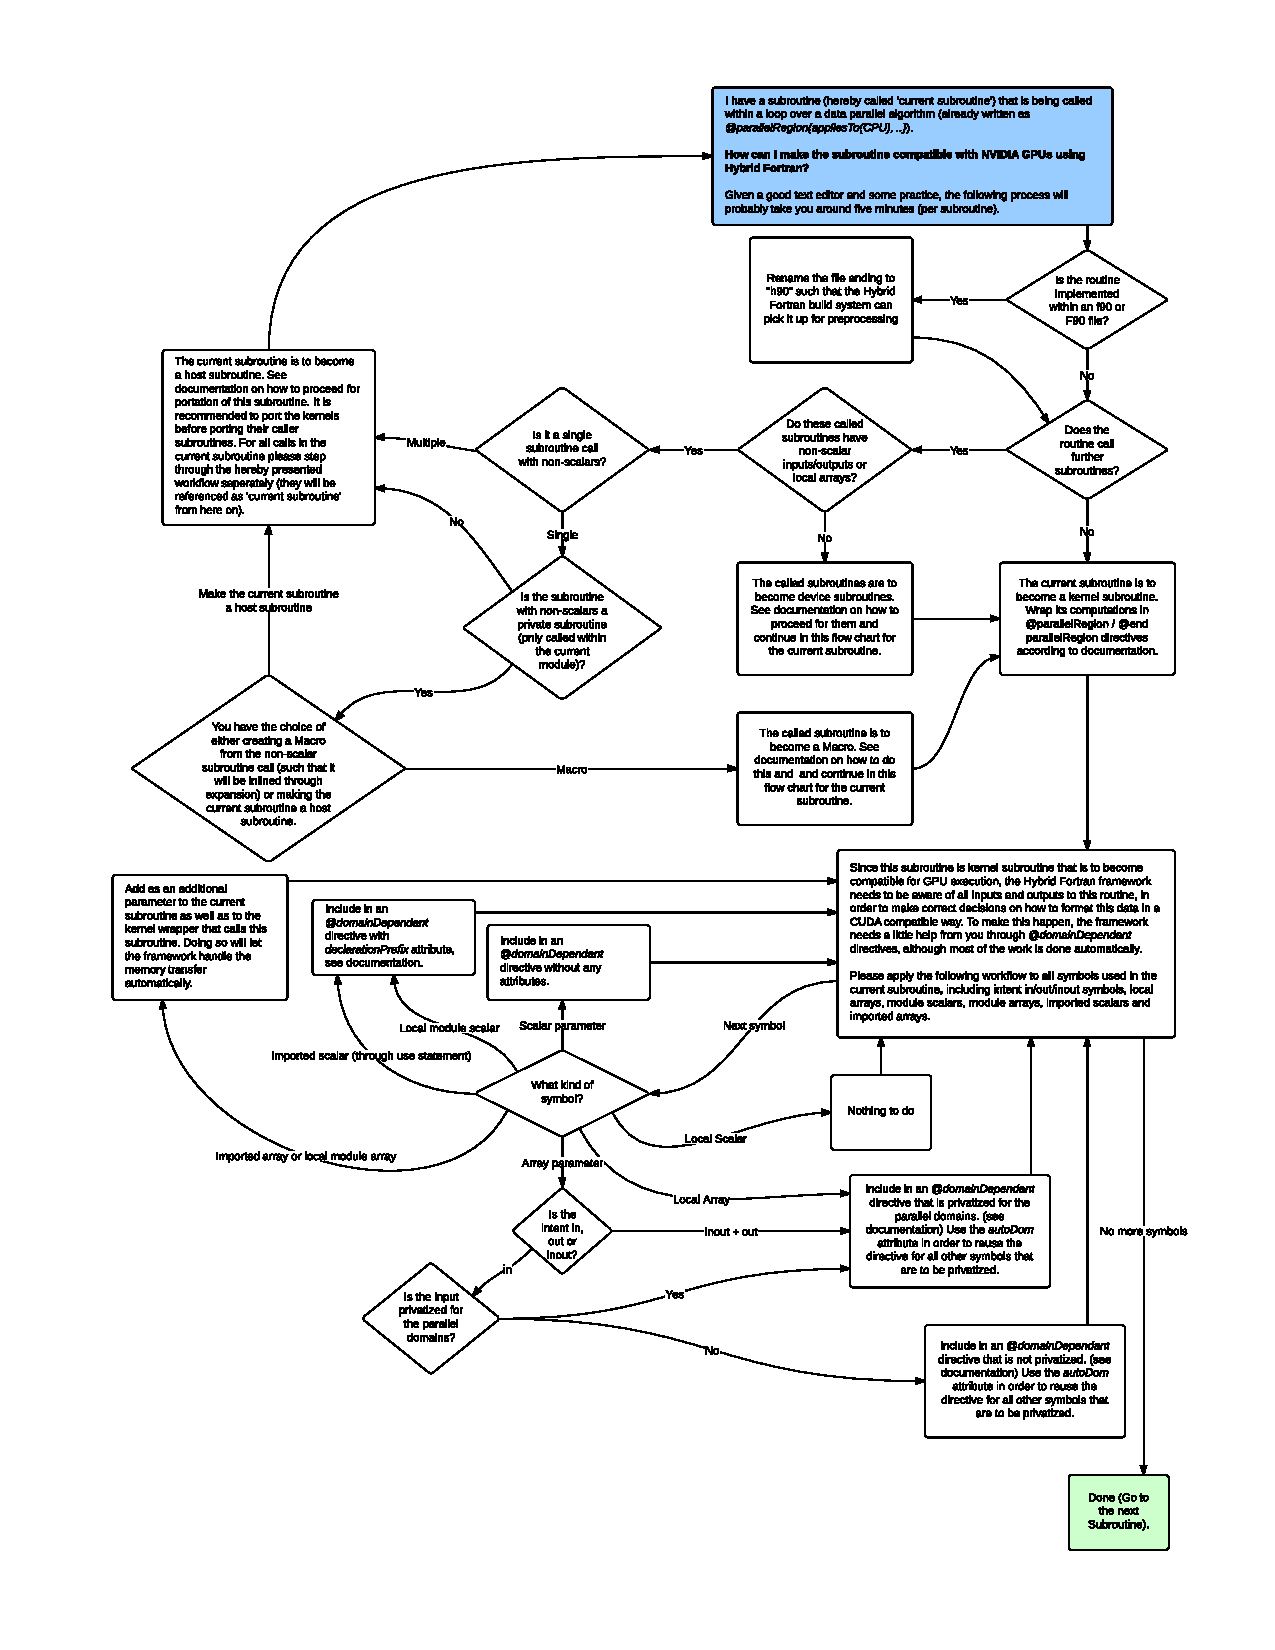
\includegraphics[width=16cm]{figures/HybridFortranGPUCompatibleCode.pdf}
  \caption [Best practices source code migration]{Best practices for a source code migration to Hybrid Fortran}
  \label{figure:bestPractMigration}
\end{figure}

Assuming that the starting point is a Fortran 90 source code for CPU, use the following guidance in order to port your codebase to \textbf{Hybrid Fortran} with the CUDA Fortran Backend. Please note: If you have many tight parallel loops in the same subroutine, you may want to start with the OpenACC backend, since it allows multiple parallel regions per subroutine. You can at a later point still easily migrate to the CUDA Fortran backend by splitting up your kernels into their own subroutine, if you find the OpenACC performance to be poor.

\begin{enumerate}
 \item Run \verb|make example| in the Hybrid Fortran root directory.
 \item Rename the new example project directory to your project name. You can also move it to any location you'd like.
 \item Delete \verb|source/example.h90| and copy in the sourcecode you'd like to hybridize using Hybrid Fortran. Please note that all loops that are to be run in parallel on CPU or GPU and their entire callgraph should be visible to the compiler in the source subdirectory. Your hybrid sources may be in an arbitrary subdirectory structure below the \verb|source| directory and may consist of \verb|f90| and \verb|F90| files. The buildsystem will find all your sourcefiles recursively and copy them into the respective build directory in a flat hierarchy.
 \item When it comes to integrating your hybrid sourcecode into a larger codebase, there are essentially two recommended options.
   \begin{enumerate}
     \item \label{enum:entireCodebase} Move the entire codebase over into the Hybrid Fortran build system. This is recommended if your build dependencies are specified in (or can easily ported to) one central Makefile.
     \item \label{enum:partOfFramework} (new since version 0.9) Move one (or later more) module of your sourcebase over into the Hybrid Fortran build system. In this case it is recommended to create a separate source directory for hybrid sources, move your code there and link its path using the \verb|SRC_DIR_COMMON| setting in \verb|MakesettingsGeneral|. Then, specify your other framework source directories using the setting \verb|FRAMEWORK_DIRS| and specify your previous main Makefile using the setting \verb|FRAMEWORK_MAKEFILE|. You should use the Makefile coming with Hybrid Fortran in the root project folder in order to interface with your build (no changes should be required other than the settings you specify in \verb|MakesettingsGeneral|. This will create separate build directories for the CPU and GPU case, copy in your \verb|FRAMEWORK_DIRS|, generate and compile the hybrid sources and then call \verb|FRAMEWORK_MAKEFILE| within the build directory. You will also need the settings \verb|FRAMEWORK_EXECUTABLE_PATHS| and \verb|FRAMEWORK_INSTALLED_EXECUTABLE_PATHS| in order to tell Hybrid Fortran which executables are being created by your build system and where you'd like them installed afterwards for testing purposes. You will need to adapt your previous build system for having moved your hybrid sources.
   \end{enumerate}
 \item In case you went with option \ref{enum:entireCodebase}, adapt your filenames containing main routines. The filename of your file(s) containing main routines need to correspond to the executable names you have specified in the \verb|EXECUTABLES| variable in \verb|MakesettingsGeneral|. E.g. if you want executables named \verb|production_exec|, \verb|test1_exec| and \verb|test2_exec|, the corresponding main files need to be named \verb|production_exec.f90|, \verb|test1_exec.f90| and \verb|test2_exec.f90|.
 \item Adjust \verb|config/MakesettingsGeneral| - the configuration options should be self explanatory.
 \item Adjust \verb|config/Makefile| by adding your hybrid source dependencies (and deleting the example). If your previous build system was already built on \verb|GNU Make| it should be possible to cut and paste your dependency definitions without change. If you would like to exclude some files or folders in your source directory from compilation (in order to integrate modules one by one), you can do this by editing the \verb|EXCEPTIONS| variable in \verb|MakesettingsGeneral|.
 \item Adjust the \verb|FFLAGS| and \verb|LDFLAGS| variables in \verb|config/MakesettingsGPU| and \verb|config/MakesettingsCPU| to reflect the compiler and linker options that are needed to compile your codebase. Please note that currently only CUDA Fortran with the Portland Group compiler \verb|pgf90| is supported and tested as the GPU implementation.
 \item Adjust the \verb|source/storage_order.F90| file according to the comments you find there. This defines storage order macros and a few other variables that Hybrid Fortran will use at the preprocessor stage. Make sure that the storage order matches a scheme that is performant on the respective target architecture - as the example shows, the \verb|GPU| variable can be used to differentiate between GPU and CPU architecture. For the GPU case, the first dimension should be the one that gets mapped to X on the threadblocks, in order for memory accesses to be coalesced. This is in turn the first dimension you specify in the \verb|domName| and \verb|domSize| attributes in your \verb|@parallelRegion| directives.
 \item Run \verb|make; make install| and run your program in order to test whether the integration of your sourcecode into the \textbf{Hybrid Fortran} build system has been successful. It should create the cpu and gpu executable versions of your program in the test directory, however the gpu version will not run on the GPU yet, since no directives have been defined so far.
 \item Integrate a test system. You can use the test scripts that have been provided with this framework (see sec.~\ref{sec:testSystem}) or use any other test system.
 \item Define the parallel regions that are to be accelerated by CPU\footnote{For example ``do'' loops that are already executed on multicore CPU using OpenMP statements.} using a \linebreak\verb|@parallelRegion{appliesTo(CPU), ...}| directive. See sec.~\ref{sub:parallelRegionDirective} for details. Rename all files that (a) contain such regions or (b) contain subroutines that are part of the call hierarchy inside those regions from \verb|*.f90| or \verb|*.F90| to \verb|*.h90|.
 \item Make sure your program still compiles and runs correctly on CPU by executing \verb|make clean; make install_cpu; [run your tests]|.
 \item (optional, you will need graphviz and pydot) Run \verb|make graphs|. You should now have a graphical representation of your call hierarchy as ``seen'' from your parallel regions upwards and downwards in the call tree.
 \item Define the subprocedures within that call hierarchy that are to be ported as GPU kernels. Fig.~\ref{figure:bestPractMigration} is designed to help you with that process. Kernel subprocedures should have the following properties:
  \begin{enumerate}
   \item They only call subprocedures from the same module.
   \item They only call one more level of subprocedures (rule of thumb).
   \item The set of these subprocedures is self enclosed for all data with depencies in your parallel domains, i.e. your data is only directly read or written to inside these to-be kernels and their callees. If this is not the case it will be necessary to restructure your codebase, e.g. put pre- and postprocessing tasks that are defined inline within higher level subprocedures into subprocedures and put them into your set of kernels.
  \end{enumerate}
 \item Make sure that callgraphs within GPU kernel subprocedures as well as kernel subprocedure callers are all defined in h90/H90 files (rename from f90/F90 where necessary).
 \item Make sure that at least the kernel callers have all the array arguments defined using \verb|intent| statements (\verb|in, out, inout|). It is recommended that all arguments in all your subroutines are defined this way, since the compiler will pick up some logical errors for you with this information. This includes pointer types as well.
 \item Analyse for all kernels which data structures they require and which of those structures are dependant on your parallel domain. Define \verb|@domainDependant| directives for those data structures within all kernels, kernel subprocedures and all intermediate subprocedures between your kernels and your CPU parallel region. See sec.~\ref{sec:archDirectives} for details. In kernel subroutines and inside kernel subroutines you will need to declare local scalars and imported data as well. See sec.~\ref{sub:domainDependantDirective} for details. See also fig.~\ref{figure:bestPractMigration}.
 \item If your kernels use arrays from the local module or imported arrays, pass them to the kernel subroutine using parameters. Use appropriate \verb|@domainDependant| directives. See sec.~\ref{sub:domainDependantDirective} for details.
 \item Imported arrays that are used in kernel subroutines and inside kernel subroutines also need to be input parameters of the kernel caller itself for appropriate automatic device data handling. That is, they need to be passed down to the kernels on two levels. Use appropriate \verb|@domainDependant| directives.
 \item Wrap the implementation sections of all your kernels with \linebreak\verb|@parallelRegion{appliesTo(GPU), ...}| / \verb|@end parallelRegion| directives. See sec.~\ref{sub:parallelRegionDirective} for details.
 \item Test and debug on CPU by executing \linebreak\verb|make clean;make build_cpu DEBUG=1| with automatic tests enabled. You can use any compatible x86 debugger here, such as PGI debugger, Intel debugger, Totalview or Allinea DDT. Please note that the debuggers will show you the line numbers of the respective \verb|F90| files, not your \verb|h90| or \verb|H90| files. The \verb|F90| files have been kept as readable as possible however, and they can all be inspected in \verb|./build/cpu/source|. Fig.~\ref{figure:bestPractDebugging} is designed to help you with this process.
 \item Switch to GPU tests debug on GPU using \linebreak\verb|make clean;make build_gpu DEBUG=1; make install_gpu; [run your tests]|. Fig.~\ref{figure:bestPractDebugging} is designed to help you with this process. The print output will help you identify problems that only exist in the GPU version. Hint: Most of the bugs that persist after having a correct CPU implementation are usually related to data dimensionalities specified using \verb|@domainDependant| directives. You should be able to trace back the error by comparing the printed output with the CPU version opened in a separate debugger window and thus identify the kernels responsible for the errors. Once you've found the offending kernels, make sure the data is correctly formatted in the specification part of the \verb|F90| file in \verb|./build/gpu/source|. If the printed output does not show the error (whose index point should be recognized in your validation / test system you've integrated before), you can change the debug data indexes in \verb|storage_order.F90|.
 \item Congratulations, you have just completed a CPU/GPU hybrid portation using \textbf{Hybrid Fortran}.
\end{enumerate}

\begin{figure}[hbtp]
  \centering  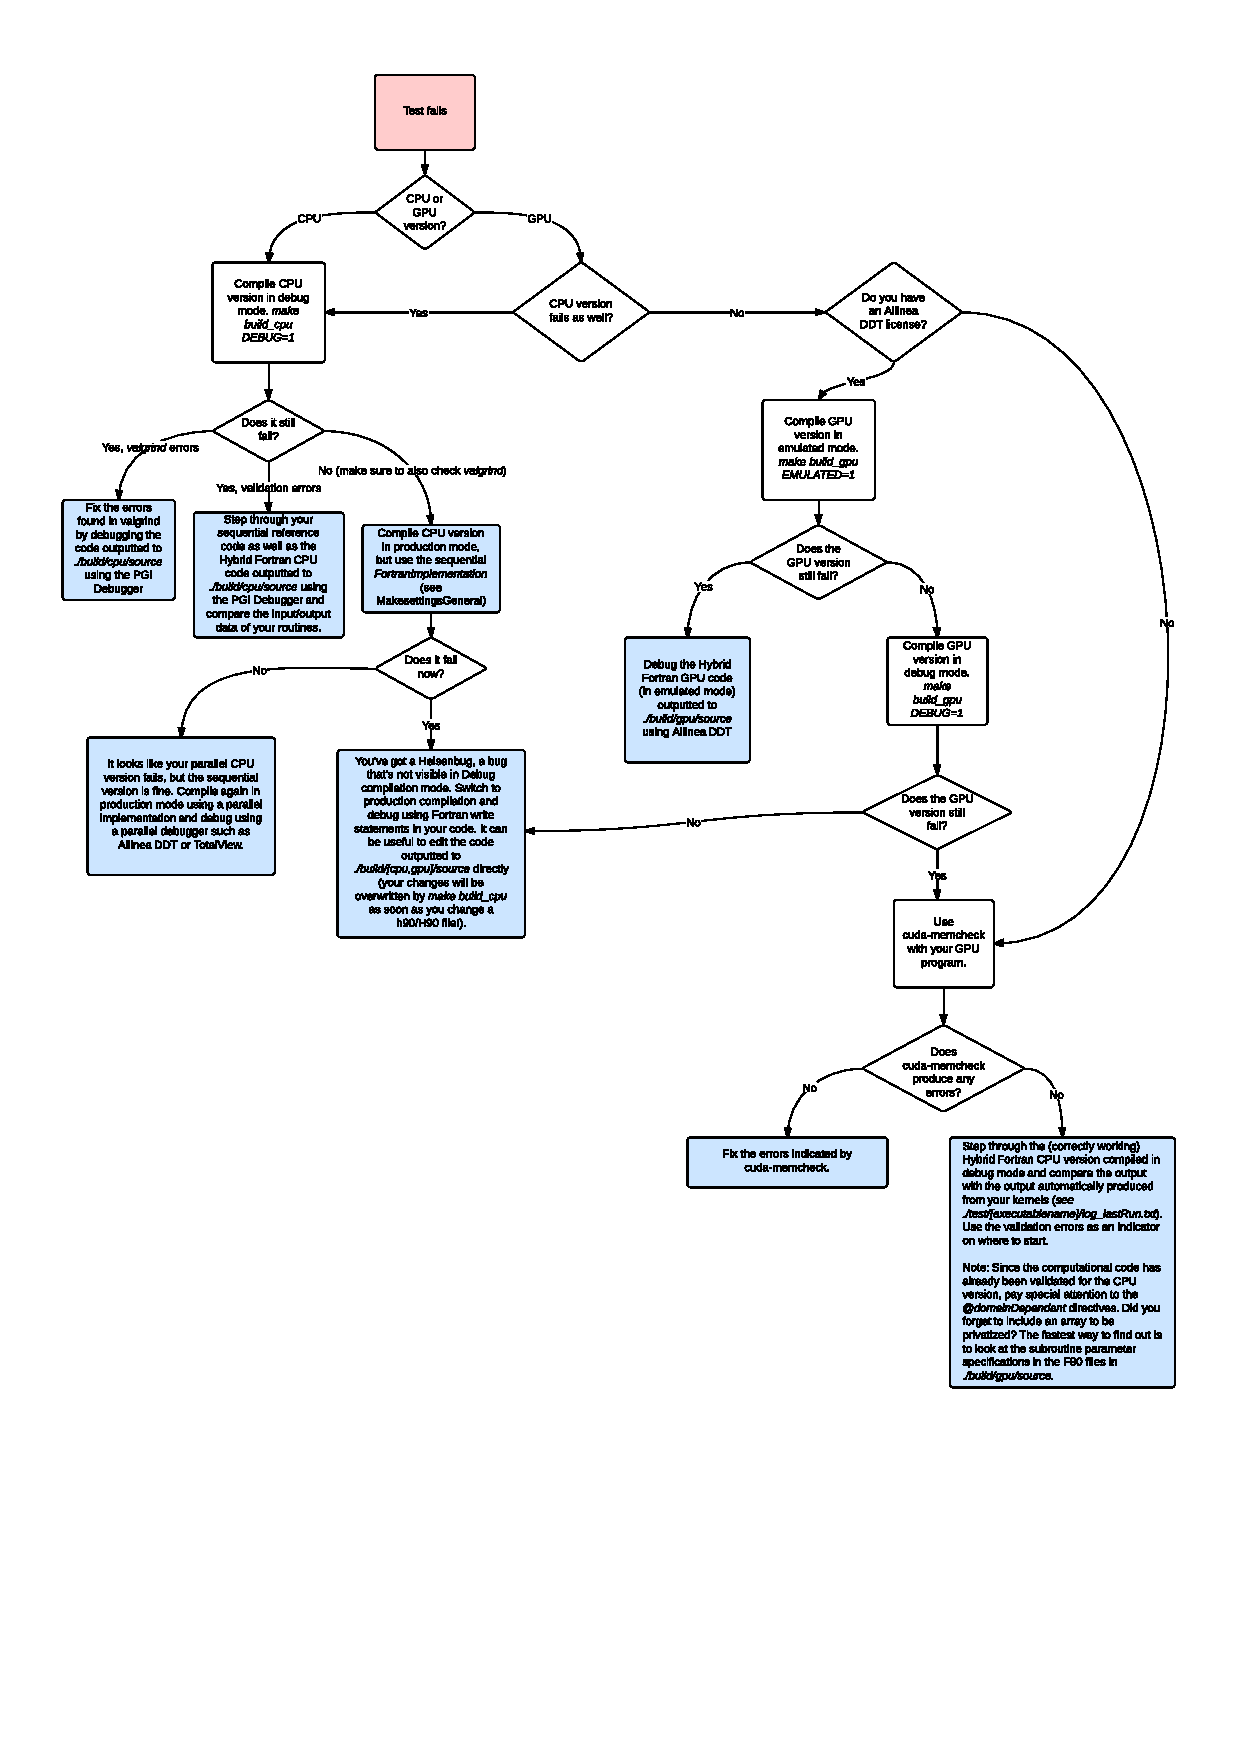
\includegraphics[width=16cm]{figures/HybridFortranDebugging.pdf}
  \caption [Best practices debugging]{Best practices for debugging Hybrid Fortran code}
  \label{figure:bestPractDebugging}
\end{figure}

